% Template for ICIP-2018 paper; to be used with:
%          spconf.sty  - ICASSP/ICIP LaTeX style file, and
%          IEEEbib.bst - IEEE bibliography style file.
% --------------------------------------------------------------------------
\documentclass{article}
\usepackage{res/packages/spconf,amsmath,graphicx}
\graphicspath{{res/imgs/},{res/plots/}}
\usepackage{hyperref}
\usepackage{url}
\newcommand{\link}[1]{\href{#1}{\textit{#1}}}
% Example definitions.
% --------------------
\def\x{{\mathbf x}}
\def\L{{\cal L}}

\renewcommand{\thesection}{\Roman{section}}
\renewcommand{\thesubsection}{\roman{subsection}}
\renewcommand{\thesubsubsection}{\alph{subsubsection}}


%prout


% Title.
% ------
\title{Website analyse}
%
% Single address.
% ---------------
\name{Romain Graux (28681700)
\thanks{Thanks to my mum.}}
\address{}
%
% For example:
% ------------
%\address{School\\
%	Department\\
%	Address}
%
% Two addresses (uncomment and modify for two-address case).
% ----------------------------------------------------------
%\twoauthors
%  {A. Author-one, B. Author-two\sthanks{Thanks to XYZ agency for funding.}}
%	{School A-B\\
%	Department A-B\\
%	Address A-B}
%  {C. Author-three, D. Author-four\sthanks{The fourth author performed the work
%	while at ...}}
%	{School C-D\\
%	Department C-D\\
%	Address C-D}
%
\begin{document}
%\ninept
%
\maketitle
%
\begin{abstract}
This report contains an analyzis of the website \link{miniclip.com}. The analyze covers three particular aspects: \textit{HTTP}, \textit{DNS} and \textit{TCP} packets.
\end{abstract}
%
% \begin{keywords}
% One, two, three, four, five
% \end{keywords}
%
\section{Introduction}
\label{sec:intro}
\subsection{Website}
\label{sub:web}
\textit{Minclip} is a free online games website. It was launched in 2001 by \textit{Robert Small} and \textit{Tihan Presbie}. The first thing to mention is that \link{miniclip.com} is automatically redirected to \link{www.miniclip.com/games/en/}, it will be explained in \textbf{\nameref{sec:HTTP}} but the analyze will be about this redirected url.
\subsection{Tools}
\label{sub:tools}
To perform the analyze, I need somme tools :
\begin{itemize}
    \item[--] \textit{HTTP}: I used \textit{Firefox Web Developper} tools.
    \item[--] \textit{DNS}: I used \textit{dig} command and \link{www.atlas.ripe.net}
    \item[--] \textit{TCP}: I used \textit{WireShark}
\end{itemize}

\section{HTTP}
\label{sec:HTTP}

\subsection{Headers}
\label{sub:headers}

As said in \nameref{sub:web}, the url \link{http://miniclip.com} is automatically redirected to \link{https://www.miniclip.com/games/en/}, this behavior is due to my browser and will not act necessarily the same on a different browser. 

First, the client will send an \textit{HTTP/2.0} request to the server that contains inter alia \texttt{Upgrade-Insecure- Requests} field set to \texttt{1}. As mention on \textit{MDN} website \cite{upgrade-insecure-request}, this field tells to the server that, if it is available, it should redirect the client to the \textit{HTTPS} version and \texttt{Status Code} returns \texttt{301}, this field means that it has to be redirected to the URL stored in the \texttt{location} field \cite{status-code-301}, so let's move to \link{https://www.miniclip.com} .

When we are on \link{https://www.miniclip.com}, the client will send an \textit{HTTP/2.0} request to the server that once again contains the \texttt{Upgrade-Insecure-Requests} field set to \texttt{1} but also contains the \texttt{Accept-Language} field set to \texttt{en} (in my case). It will act the same as aforementioned, the server will set the \texttt{Status Code} field to \texttt{301} and set the \texttt{location} field to \link{https://www.miniclip.com/games/en/} and we are redirected.

Then the client send the \textit{request header} to the server that will return a \texttt{200 Status Code} and the
source code of the page stored in the body, the client is now able to load the content.

\subsection{Resources types}
\label{sub:res}

When the client as load the HTML, he needs to load all the content linking in the file from different domain (\url{www.youtube.com}, \url{apis.google.com}, \url{static.miniclipcdn.com}, , ...). For that, it sends requests to all server that contains data, for the main page, it sends 94 requests. As we are on \textit{HTTP/2.0}, \textit{multiplexing} is used and one connection is established between the client and a domain containing data the client needs to download.
% The website need a lot of images to illustrate games you can choose.

Resources loading from \textit{miniclip} are not only loaded from one \textit{miniclip} domain. For example, resources are loaded from \url{static.miniclipcdn.com}, \url{static2.miniclipcdn.com} or \url{static3.miniclipcdn.com}. This behavior is due to the browser that has a hard limit on the number of parallel requests it can execute to the same domain at the same time. Here the client is able to load three times more information at the same time.

\begin{figure}[h]
    \centering
    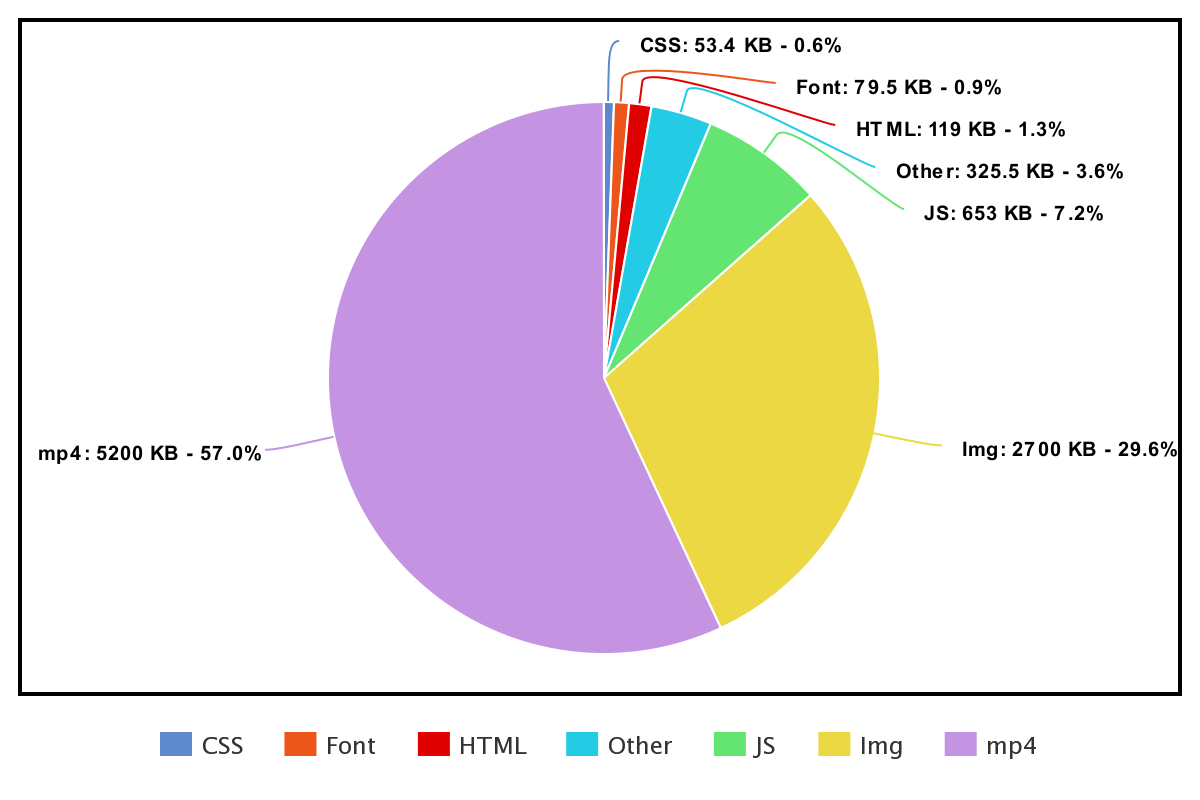
\includegraphics[width=0.45\textwidth]{res/imgs/resources.png}
    \caption{Resources types}
    \label{fig:res}
\end{figure}

\subsection{Cookies}
\label{sub:cookies}

\subsubsection{Types}

There are a lot of cookies used to track the client along all the website. They can be set by \textit{miniclip} itself or other website when request are made (IFrame or JS). There are cookies for advertisment that are set in normal mode or 'incognito' mode (\texttt{$\_\_$gads} is a Google cookie preventing the same ads from being shown to the client too many times, \texttt{$\_$fbp} is a Facebook cookie used too set third-party advertisement,...). There are cookies for identifying the client (). There are also cookies about client information such as localisation, language, ... (\texttt{$\_$country$\_$code} is used to indentify the client country, \texttt{$\_$eu$\_$cookie} is used to identfy if the client is in Europe, \texttt{$\_$language$\_$code} is used to identify the language that has to be chosen by the server, ...)

\subsubsection{Weird behavior}

When the client load the website free from cookies (First time or in incognito tab), \texttt{$\_\_$gads} and \texttt{$\_$fbp} cookies don't appear anywhere, that means that they are not set anywhere when the ressources are loaded. In fact, they are set from a \textit{JavaScript} file,the \texttt{$\_\_$gads} cookie is set in the Javascript contained in \url{https://securepubads.g.doubleclick.net/gpt/pubads_impl_modern_2019112101.js} the \texttt{$\_$fbp} cookie is set in \url{https://connect.facebook.net/signals/config/1451566791782906?v=2.9.14&r=stable}.
% On \textit{miniclip}, there are 4 different cookies owners: \textit{miniclip, google, youtube} and \textit{facebook}.
% \begin{itemize}
%     \item[--] \textbf{miniclip}
%     \begin{itemize}
%         \item \texttt{\_country\_code, \_eu\_cookie} : Contain localisation informations.
%         \item \texttt{\_fbp} : It is a Facebook cookie that is used for advertisment.
%         \item \texttt{\_\_ads} : It is a Google cookie that is used to not showing the client too much time same advertisments.
%     \end{itemize}
%     \item[--] \textbf{facebook}
%     If the client have already registered, he has these cookies \cite{facebook-cookies}:
%     \begin{itemize}
%         \item \texttt{act} : Tells when the user logged in.
%         \item \texttt{c\_user} : Contains the facebook login ID.
%         \item ...
%     \end{itemize}
%     When the user has open an incognito tab, these cookies are session cookies, instead, they expire in 90 days.
%     \item[--] \textbf{google}
%     \item[--] \textbf{youtube}
% \end{itemize}

\subsection{Ports}
\label{sub:ports}

Every HTTPS request is established over the port 443 and every HTTP request is established over the port 80.

\section{DNS}
\label{sec:DNS}

% ns-251.awsdns-31.com
% ns-867.awsdns-44.net
% ns-1518.awsdns-61.org
% ns-1577.awsdns-05.co.uk

% Miniclip has 4 DNS : {ns-251.awsdns-31.com}, {ns-867.awsdns-44.net}, {ns-1518.awsdns-61.org} and {ns-1577.awsdns-05.co.uk}. All can be accessed either in IPv6 or IPv4.

Miniclip uses 4 different IPv4 addresses $13.225.233.84$, $13.225.233.19$, $13.225.233.7$ and $13.225.233.45$. 

\section{TCP}
\label{sec:TCP}





% References should be produced using the bibtex program from suitable
% BiBTeX files (here: strings, refs, manuals). The IEEEbib.bst bibliography
% style file from IEEE produces unsorted bibliography list.
% -------------------------------------------------------------------------
\bibliographystyle{res/bib/IEEEbib}
\bibliography{res/bib/strings,res/bib/refs,res/bib/fields}

\end{document}
